\documentclass[a4paper,12pt]{ctexart}

\setlength{\parskip}{0.5em}

\setcounter{secnumdepth}{-2}

\usepackage{endnotes}
\usepackage[stable]{footmisc}
\renewcommand{\notesname}{注释}

\usepackage{changepage}
\usepackage{hyperref}%设置超链接

\usepackage{zref-perpage}
\zmakeperpage{footnote}

\usepackage{pifont}
\newcommand*\dingctr[1]{%
  \protect\ding{\number\numexpr\value{#1}+171\relax}}
\renewcommand*\thefootnote{\dingctr{footnote}}

\usepackage{xeCJK}
\setCJKmainfont[ItalicFont=SourceHanSerifCN-ExtraLight,BoldFont=SourceHanSerifCN-Bold]{SourceHanSerifCN-Regular}

\usepackage{graphicx}

\usepackage{nomencl}
\makenomenclature
\renewcommand{\nomname}{德中译名表}

\title{\marginpar{459}\Huge 共同主义政党宣言}
\author{卡·马克思\quad 弗·恩格斯著\\王苏谈译}
\date{}

\begin{document}

\maketitle
\thispagestyle{empty}
\newpage

\section{譯者序言}

卡·馬克思、弗·恩格斯二人起草的這本《宣言》,德文初版於1848年2月於倫敦。而見諸世人的首份漢文全譯版,則有賴於陳望道先生的翻譯工作。該漢譯版初版於1920年8月於上海。陳望道先生的諸版本,對於馬克思學說在中國的傳播,意義非凡。然而可惜,受制於文獻來源等方面,該版本主要使用的1888年英譯本(由赛米尔·穆尔譯、弗·恩格斯校訂並加註)和(疑)1906年日譯本(堺利彦訳、幸徳秋水譯)。

此後,在中國大陸,承擔《宣言》編譯工作的,主要是共產黨人身份的譯者,如華崗、成仿吳、徐冰、博古等人,或是官方機構,如中央編譯局。迄今較知名的非共產黨人身份的譯者,唯有陳瘦石一人而已。

一些讀者可能會有疑問:既然官方已經負責了《宣言》(以及其他經典著作)之翻譯工作,為何還要重譯《宣言》呢,不是多此一舉麼?

筆者重譯《宣言》的動機主要在於:

首先,衆所周知,翻譯外文文獻,最好是直接依靠原文,而不可倚重譯文。我國向來的譯本,要麼直接用的其他語種的譯文,要麼雖用的或參考的有原版,然受到了各種譯文之深刻影響。那麼,就有必要完全從德文的原代碼,重新乾乾淨淨地編譯一遍。

筆者參考的是MIA網站上錄入的德文網頁版,之後用MEW的德文版初步校對了頁碼、腳註等部分。由於精力有限,考慮日後逐步地對照上述二個德文版,確保文本一致。

其次,目前國內的《宣言》的編譯工作,實際上是被官方機構所壟斷了。我國《宣言》研究也就陷入了嚴重的路徑依賴。舊官譯本所含的形形色色的錯誤,就這樣持續地存在,並且被讀者無意識地接受。要想爲《宣言》乃至其他經典作品的翻譯,打破這樣的暮氣沉沉的僵局,打開別樣的朝氣勃勃的新局,則筆者作為政治上獨立的個體,特別是作為革命的馬克思主義者,來重譯《宣言》,就顯得頗有必要了。

而且,筆者此前曾重譯過德文版的《[政治經濟學批判]導論》,發現問題不少,特別是起底了所謂“邏輯與歷史相統一”,證明它不過是一種偽造理論,而發揮了馬克思自己真正的辯證方法,「環節式上升法」,那麼,我就有理由懷疑:《宣言》中有沒有一些嚴重的問題呢。說實話,我重譯《宣言》的工作,在我完成当时的《導論》之翻譯和研究之前,就已經開始了。當時就發現不少問題,更堅定了我的志願:總要自己把這個《宣言》給翻譯出來才行。

然後,我是如何重新接續我的翻譯進度的呢?契機是我某次去南京雨花臺景區,發現那裏有一面《宣言》的書法牆。我憶起了我自己的翻譯工作,就此下定決心,一定要儘快重啓我的進度,並爭取在2021年7月之前譯出來。

所以現在讀者面前就呈現了這麼一個新的漢譯本。

我的譯本有一些比較重要的特點,現在給大家講一下:

(一)底本是德文版。之後我會進一步確認相關原文,並進一步參校其他譯本,如日、英譯本。

(二)專門製作了德中對照的譯名表。對學術的編譯工作而言,這個部分不可或缺。然而衆所周知,我國馬克思主義著作的官方譯本根本沒有這樣的東西。

(三)革命的馬克思主義的立場。1890年恩格斯編輯過的德文原版,已經是二位作者所修改的最後的定版了。從純粹的文字層面上講,這個版本無法再做什麼重大的改變。但這些文本不是與世隔絕的靜止的東西,相反總處於與現狀相聯繫相互動的運動的狀態。(前者屬於知性的舊唯物主義,而後者屬於辯證法。)更不必說,其他的譯本,自然是經常處在變動之中,因為其本身相對於原本必然具有一種特殊性,即:譯本不是原本,而經常要據原本來改善譯本之翻譯質量。而且,翻譯的過程天然包含著理解的過程,而理解的方式,自然根據著譯者所處的社會階段而有其特殊性。這裏,就要求譯者有一種革命的、普遍的立場,能夠以譯者自己在特殊形式上的譯文,儘可能體現原作者在普遍意義上的原文,就是說展現原文本身的普遍內容,並且,同時要尊重原文當時的時代環境。所以,筆者作為革命的馬克思主義者,無官方背景,有必要學識,或能更好地承擔這樣的任務:從理論立場上儘可能領會馬克思他們的學說,並且在實際的翻譯上充分體現原文中的普遍內容。

其他的變動不居的東西,比如有待完善的部分或環節、最近的進度等等,我想不必在序言這裏講。進一步的完善,以及全面的、逐字逐句的解讀,我日後也會逐步跟進。若讀者知曉程序設計中的迭代思想,也就不難理解我這種做法了:在程序接近全面完善之前,我們可在它較完善時就發布出來,日後再不斷地完善它。

期待諸位讀者能從我的新譯本中得到一些新東西。

\newpage
\tableofcontents
\thispagestyle{empty}

\newpage
\thispagestyle{empty}
\marginpar{460}

\begin{center}
写於1847年12月至1848年1月。

印刷并作为单册出版於1848年2月-3月於伦敦。

当前的版本以最后由\\弗里德里希·恩格斯所处理的1890年德文版为基础。
\end{center}

\begin{adjustwidth}{2.5cm}{2.5cm}
\vfill 在脚注中,1848、1872、1883年诸德文版各不相同的异文已被注明,只要这些异文涉及内容。起草者关於《宣言》的全部前言,我们都当作附件放在当前卷之末尾。\footnote{本汉译版未添加相关前言。——译注}
\end{adjustwidth}

\newpage
\thispagestyle{empty}
\vspace*{80pt}
\centerline{
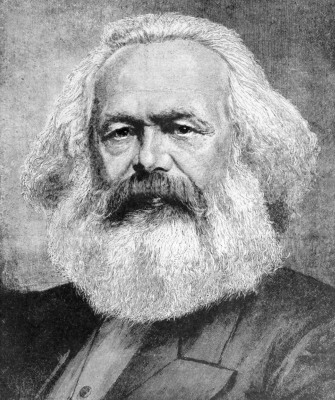
\includegraphics[width=0.8\textwidth]{0111207237-Marx.jpg}
}
\begin{center}
卡尔·马克思,革命家,经济学家,《宣言》作者之一。
\end{center}

\newpage
\setcounter{page}{1}

\marginpar{461}一個惡灵[Gespenst],出没於歐洲。这个惡灵,名爲共同主義。旧歐洲所有勢力都结盟起來,进行神聖的畋猎,以對抗这個惡灵。這些势力中,有教宗和沙皇,梅特涅和基佐,法兰西激進派和德意志警察。

哪個反對党,不是被掌權的對手詆譭成共同主義的呢?而这些反對党,难道不是如同其反動對手那样,又把共同主義这个打上烙印的斥责,转擲给更進步的反抗民众?

此二者,皆源出这一事实。

共同主義已然被歐洲所有势力公認为一种势力。

现在正是時候,共同主義者要将他们的观察方式,他们的诸多目的,他们的诸多倾向,向全世界公开陳述,并以党自己的宣言,抵制那[dem]\footnote{(1848年版) den[这里是改变了德语的冠词。以下类似情况不再专门提示。——译注]}共同主義惡灵的流言。

为此目的,最广泛诸國之共同主義者集會於倫敦,起草如下宣言,发表之以英语、法语、德语、意大利语、法兰德斯语和丹麥语。

\newpage

\marginpar{462}\section[一、资产者与无产者]{一、资产者与无产者\protect\endnote{资产阶级是被理解为现代诸资本家之阶级,它是社会性的生产资料之占有者,并且利用雇佣劳动。无产阶级是被理解为现代雇佣工人之阶级,因不占有自己的生产资料,则依赖於出卖劳动力以维生。[恩格斯在1888年英文版中的注释。]}}

迄今所有社会之历史\endnote{Das heißt, genau gesprochen, die \textit{schriftlich} überlieferte Geschichte. 1847 war die Vorgeschichte der Gesellschaft, die gesellschaftliche Organisation, die aller niedergeschriebenen Geschichte vorausging, noch so gut wie unbekannt. Seitdem hat Haxthausen das Gemeineigentum am Boden in Rußland entdeckt, Maurer hat es nachgewiesen als die gesellschaftliche Grundlage, wovon alle deutschen Stämme geschichtlich ausgingen, und allmählich fand man, daß Dorfgemeinden mit gemeinsamem Bodenbesitz die Urform der Gesellschaft waren von Indien bis Irland. Schließlich wurde die innere Organisation dieser urwüchsigen kommunistischen Gesellschaft in ihrer typischen Form bloßgelegt durch Morgans krönende Entdeckung der wahren Natur der Gens und ihrer Stellung im Stamm. Mit der Auflösung dieser ursprünglichen Gemeinwesen beginnt die Spaltung der Gesellschaft in besondre und schließlich einander entgegengesetzte Klassen. \textit{[Anmerkung von Engels zur englischen Ausgabe von 1888 und zur deutschen Ausgabe von 1890.]} Ich habe versucht, diesen Auflösungsprozeß in  „Der Ursprung der Familie, des Privateigenthums und des Staates“ zu verfolgen; zweite Auflage, Stuttgart 1886. \textit{[Anmerkung von Engels zur englischen Ausgabe von 1888.]}},皆为阶级斗争的历史。

自由民与奴隶,贵族与平民,领主与农奴,行会市民与帮工,简言之,压迫者与被压迫者,相互间处於持续的对立之中,进行着不间断的,时而隐蔽时而公开的斗争,而这一斗争,总是以整个社会之革命的改造而告终,或者是斗争的诸阶级同归於尽。

以往的历史诸时代中,几乎到处都能发现:社会之彻底地划分为不同等级,社会的诸地位之多种多样的分层。在古罗马,有\marginpar{463}贵族,骑士,平民,奴隶;在中世纪,有封建主,臣仆,行会市民,帮工,农奴,此外,在几乎每一阶级中,又皆有特殊的诸阶层。

从封建社会的灭亡中产生出来的现代资产阶级社会,并未消灭阶级对立。它仅仅拿新的阶级,新的压迫条件,新的斗争形态,代替了旧的。

我们的时代,资产阶级的时代,却有一个特征,即它已简化阶级对立。整个社会日渐分裂为二大敌对的阵营,二大直接对峙的阶级:资产阶级与无产阶级。

%2021-04-18

从中世纪之农奴产生出来最初的那些城市[Städte]之桩内市民;从这一桩内市民关系中发展出最初的资产阶级之诸元素。

美洲的发现,非洲的绕航,给势均力敌[aufkommenden]的资产阶级创造了新的优势。东印度和中国的市场,美洲的殖民化,同殖民地的交流,交换手段和商品的增加,普遍地使贸易、航运、工业得到无可估量的繁荣,从而使革命的因素,在崩溃中的封建社会里,得到快速的发展。

以前的封建的或行会的工业之经营方式,对於随着新[neuen]\footnote{(1848、1872、1883年版)那新的}市场而增长中的需求,不再足够。工场手工业取而代之。行会师傅为工业的中间等级所排挤;形形色色的团体之间的分工,在单个作坊本身内的分工面前消失了。

但市场总在扩大,需求总在上涨。甚至工场手工业也不再足够。於是蒸汽与机组革新了工业生产。工场手工业被代以现代大工业,工业的中间等级被代以工业的百万富翁,所有工业大军的首领,现代的资产者。

世界市场由美洲的发现而酝酿,由大工业而确立。世界市场使贸易、航运、陆上交流得到无可估量的发展。这\marginpar{464}又反作用於工业的扩展,而在同等程度上,哪里工业、贸易、航运、铁路扩展,在同等程度上资产阶级也发展,增殖其诸资本,把所有从中世纪流传下来的阶级挤到幕后。

由此我们可见,现代资产阶级本身,是长期的发展过程之产物,是生产方式、交往方式上一系列变革之产物。

%2021-04-18

资产阶级每个这样的发展阶段,都伴随着\footnote{(1888年版)补充:这一阶级}相应的政治进步。封建主统治下的被压迫等级,公社[Kommune]\endnote{„Kommune“ nannten sich die in Frankreich entstehenden Städte, sogar bevor sie ihren feudalen Herrn und Meistern lokale Selbstverwaltung und politische Rechte als „Dritter Stand“ abzuringen vermochten. Allgemein gesprochen haben wir hier als typisches Land für die ökonomische Entwicklung der Bourgeoisie England, für ihre politische Entwicklung Frankreich angeführt. \textit{[Anmerkung von Engels zur englischen Ausgabe von 1888.]}\\So nannten die Städtebürger Italiens und Frankreichs ihr städtisches Gemeinwesen, nachdem sie die ersten Selbstverwaltungsrechte ihren Feudalherren abgekauft oder abgezwungen hatten. \textit{[Anmerkung von Engels zur deutschen Ausgabe von 1890.]}}中武装的和自治的联合体[Assoziation]\footnote{(1848、1872年版)诸联合体},这儿是独立的城市共和国\footnote{(1888年版)补充:(如在意大利和德意志)},那儿是君主国之第三纳税等级\footnote{(1888年版)补充:(如在法兰克帝国)},后来在工场手工业时期,是等级制的或专制的君主国中反对贵族的均势\footnote{(1888年版)补充:并且},特别是大君主国之首要基础,最终,自从大工业和世界市场建立起来,它在现代的代议制国家中,就夺取了独占的政治的统治。现代的国家权力机关[Staatsgewalt],不过是一种委员会,以管理整个资产者阶级的公共业务。

资产阶级在历史上,曾扮演极度革命的角色。

%2021-04-19

资产阶级,在它取得统治的地方,把一切封建的、家长制的、田园般的关系都给破坏了。它把形形色色的封建束缚,之使众人依赖於其天然的尊长者,给无情撕碎了,并且在人与人之间,再也没有任何其他联系,只剩下赤裸裸的利益,剩下冷酷的「现金交易」。虔诚的狂热,骑士\marginpar{465}的热忱,小市民的忧郁,对这些东西的神圣敬畏,都被它溺死在自私自利的算计之冰水中。它把个人的尊严消解为交换价值,并把数不尽的书面确认的、确实获得[wohlerworbenen]的自由,代替以\textbf{一种}没良心的贸易自由。一言以蔽之,它把由宗教的、政治的幻觉所掩盖的剥削,代替以公然、无耻、直接、露骨的剥削。

资产阶级对迄今所有的令人崇敬并以虔诚的战兢来看待的诸多职业,剥夺了它们的圣光。它把医生、法学家、教士、科学界人士,变成它有偿的雇佣劳动者。

资产阶级扯下家庭关系它的多情善感的面纱,将之归结为纯粹的货币关系。

%2021-04-20

资产阶级已经揭露:那野蛮的出力,被反动派在中世纪如此这般极为赞赏,[却]已发现最极端的懒汉是其合适的补充。它已率先指出,人们的活动可以干成什么。它完成了完全不同的奇迹之作,异於埃及金字塔、罗马水道、哥特式大教堂,它完成了完全不同的远征,异於民族大迁徙和十字军东征。

资产阶级无法生存,除非对生产工具[Produktionsinstrumente],从而对生产关系,从而对全部社会关系,不断地革命化。旧的生产方式[Produktionsweise]的一成不变的情况,相反地是所有以往的工业阶级首要的生存条件。生产之不断变革,所有社会状况之不间断的动荡,永远的不确定与运动,使得资产者时代在所有其他\footnote{(1848、1872、1883年版)以往}时代面前凸显出来。一切牢固、僵硬的关系,连同其随从,即历史悠久的观念和观点,都被消灭,一切新建立的东西都变得过时,来不及僵化。一切等级的东西、固定的东西都蒸发了,一切神圣的东西都被亵渎了,而人终究被迫以清醒的眼光,来评价他们的社会地位,他们相互间的关系。

产品对始终膨胀的销路的需求,赶着资产阶级走遍全球。它必须四海定居,遍地扩张,到处建立联系。

%2021-04-20

\marginpar{466}资产阶级由於他们的[ihre]\footnote{(1848年版):die}开发世界市场,已使所有国家的生产与消费都成为世界主义的。令反动派们极为遗憾的是,资产阶级把国家的工业基础连根铲除。古老的国家工业已被毁灭,而且每日还在被毁灭。古老的国家工业被排挤以新的工业,这种新的工业的采用对於所有文明国家来说都生死攸关;被排挤以这样的工业,它们所加工的不再是本国的原料,而是属於最边鄙地带的原料,且其工业产品的消耗不仅是在本国,而且是在所有大洲。那旧的、由国产货来满足的需要,代替以新的需要,这种需要要求将最遥远的地方和气候之产品当作其满足。旧的地方的、国家的自给自足与自成一体,代替以全面的交往和诸国互相的全面依赖。就像对於物质生产那样,对於精神生产亦如此。各国的精神成果,成为公共财产。民族的片面性与狭隘性越来越不可能,并且由许多民族的、地方的诸文献,得以形成一个世界文献。

资产阶级靠一切生产工具的快速改良,靠无限方便的交流,将一切的、甚至最野蛮的民族,拽进了文明之中。资产阶级的商品之低廉价格就是重炮,资产阶级以它来彻底摧毁一切万里长城,强迫野蛮人最顽固的仇外来投降。它强迫一切民族,学会资产阶级之生产方式,如果这些民族不想覆灭的话;它强迫这些民族,将所谓的文明引入它们自己那里,即是说,变成资产者。一句话,资产阶级根据它自已的面貌,来创造一个世界。

资产阶级使农村从属於城市的统治。它创建了诸多庞大的城市,使城市的人口数相对於农村的人口数,在高的等级上增长,因而使相当大部分的人口,摆脱了农村生活的愚昧状态。正如它使农村从属於城市,它已使野蛮、半野蛮国家[Länder]从属於文明国家,使农业人群从属於资产者人群,使东方从属於西方。

%2021-04-22

资产阶级日益消灭生产资料、财产、人口的分散。它聚集\marginpar{467}人口,集中生产资料,并汇集财产於少数人之手。由此而来的必然结果,就是政治的集中。独立的、几乎仅结盟的诸省,连同形形色色的利益、法律、政府、关税,被精简为\textbf{一个}国家、\textbf{一个}政府、\textbf{一套}法律、\textbf{一个}国家的阶级利益、\textbf{一条}海关线[Douanenlinie]\endnote{(MIA在线网页德文版)(Douane:法语。即海关。)}。

资产阶级在其几乎不到百年的阶级统治中所创造的生产力,相比所有过去的世代加在一起,都是更大规模的、更庞大的。对自然力的征服,机组,化学之应用於工农业,汽船,铁路,电报,整个整个大洲的开垦,河流的通航,完全凭空而出的人口——以往哪个[welches frühere]\footnote{(1848年版)welch früheres[哪个以往]}世纪能想到:在社会劳动的母腹之中,潜藏有这般的生产力。

由此[also]\footnote{(1848年版)可是[aber]}我们已经看出:生产资料与交通工具[Die Produktions- und Verkehrsmittel],资产阶级以之为基础而成长出来者,是在封建社会里诞生的。在这些生产资料与交通工具之发展之某个确实的阶段[Stufe]上,封建社会在其中生产、交流的那些关系,农业与工场手工业之封建组织,一言以蔽之,封建的财产关系,不再适应於已经发展的生产力。它们是阻碍生产,而非促进。它们变成了同等程度的束缚。它们必须被挣脱,并且已经被挣脱。

取而代之者,是自由竞争,以及适应於它的社会的、政治的体制,以及资产阶级之经济的、政治的统治。

%2021-04-23

在我们眼下,类似的运动在推进着。资产阶级的生产关系、交往关系,资产阶级的财产关系,现代资产阶级社会,幻化出来了如此强大的生产资料、交通工具[Produktions- und Verkehrsmittel],正像一位巫师,召唤过来冥界之力,却再也无法掌控之。数十年来,工业和贸易之历史,不过\footnote{(1848年版)补充:仍然}是这些起义之历史,[这些起义]即现代生产力反对现代生产关系、反对财产关系,而这些[关系]正是资产阶级及其统治的生活条件。列举出商业危机就足够了。商业危机以其周期性的复归[Wiederkehr],总是预示着整个资产阶级社会之存在都成了\marginpar{468}问题。在商业危机中,不仅一大部分生产出来的产品,而且\footnote{(1848年版)补充:甚至}一大部分已经创造的生产力,经常被毁灭。在危机中,爆发出一种社会的大流感。这种大流感,於所有以往时代而言,都会显得是一种荒唐事——这就是生产过剩的大流感。社会发现:自己突然回復到一种短暂的野蛮之状态;似乎是一次饥荒,一场普遍的歼灭战\footnote{(1848年版)毁灭战},中断了其所有生活资料[Lebensmittel];工业、贸易似乎毁灭了。为什么呢?是因社会占有过剩的文明,过剩的生活资料,过剩的工业,过剩的贸易。供社会使用的生产力,不再提升\footnote{(1848年版)补充:资产阶级的文明和}资产阶级的财产关系;相反,对那些关系而言,生产力变得[过於]强大,生产力为那些关系所阻碍;而生产力只要克服这些阻碍,就会把整个资产阶级社会带入混乱之中,危及资产阶级的财产之存在。资产阶级的关系已然变得狭隘,容纳不了由它们生出的财富。\iffalse 2021-04-24\fi ——资产阶级如何克服这种危机呢?一方面靠强制毁灭大量生产力;另一方面靠占领新市场、更彻底地开发旧[alter]\footnote{(1848、1872年版)der alten}市场。然后呢?由此,资产阶级就酝酿了更全面、更严重的危机,而减少了预防危机的手段。

那些武器,资产阶级借以曾将封建主义打倒在地的,如今对准了资产阶级自己。

然而资产阶级不仅锻造了这些武器致之於死地者;它还产生了一些人[Männer]来运用这些武器——现代工人,\textbf{无产者}。

资产阶级,也即资本,发展到什么程度,无产阶级,现代劳动者之阶级,就发展到什么程度。无产阶级要想如此长期地生活,就要找到工作,而要想找到如此长期的工作,他们的劳动就必须增殖资本。这些工人必须逐份出售自己者,就是一种商品,就如同每种其他货品,因而同等地遭受全部的竞争涨跌、市场波动。

无产者的劳动,由於机组的扩展、劳动的分工[die Teilung der Arbeit],已失去了一切独立的性质,因而对[die]\footnote{(1848年版)den}劳动者失去一切吸引力。工人变成了纯粹的机器之附件,只被\marginpar{469}要求最简单、最单调、最易学的操作。因而工人引起的费用,几乎仅限於生活资料。对他自己的维生与其种族[Race]的繁衍来说,这些生活资料是必需的。商品、因而也包括劳动\endnote{In späteren Werken verwandten Marx und Engels an Stelle der Begriffe „Wert der Arbeit“ und „Preis der Arbeit“ die von Marx eingeführten genaueren Begriffe „Wert der Arbeitskraft“ und „Preis der Arbeitskraft“.},其价格却都等於其生产费用。劳动变得怎样讨厌,工资就怎样下降。不仅如此,机组与分工[Teilung der Arbeit]怎样加强,劳动的量\footnote{(1888年版)负担}也就怎样增加,这来自工时之延长,来自既定时间内所要求的劳动之增加,诸机器之加快运转云云。

%2021-04-25

现代工业变家长制师傅之小作坊,为工业资本家之大工厂。工业群体,一起挤在工厂里,像士兵那样被组织起来。他们被当作普通的[gemeine]工业兵,受到士官和军官的某种彻底的等级制之监管。他们不仅仅是资产阶级之奴隶,资产者国家之奴隶,还每日每时都受奴役於机器、监工,且首先受奴役於那[den]\footnote{(1848年版)dem}单个的制造的[fabrizierenden]资产者自己。这个暴政越是公然宣称收入是它的\footnote{(1848、1872、1883年版)补充:最终的}目的,它就越自私、尖刻、乖张。

手工作业越少要求技巧和出力,换言之,现代工业越发展,则男人[Männer]之劳动就越多为女人\footnote{(1848年版)补充:和儿童}的劳动所排挤。性别、年龄的区别,对工人阶级再也没有更多的社会效力了。只是还有些劳动工具,视年龄、性别而产生各不相同的费用罢了。

工厂主对工人的剥削到达一定程度,工人得到现金支付的劳动工资,那么另一部分资产阶级就来纠缠他,即房东、商贩、当铺[Pfandleiher]\footnote{(1848、1872、1883年版)Pfandverleiher}等等。

以前的小的中间等级,小的工业家、商人与食利者,手工业者与农民,所有这些阶级都滑落为无产阶级,有的是由於其小资本不足以经营大工业,而无力同大资本家相竞争,有的是由於其技巧对新的生产方式变得无效。因此无产阶级就增补以人口的所有阶级。

%2021-04-26

\marginpar{470}无产阶级历经各不相同的发展阶段。它自存在以来,就为反对资产阶级而斗争。

起初是单个工人,然后是一个工厂的工人,然后是一个地区的一个劳动部门的工人,为反对直接剥削他们的单个诸资产者而斗争。工人们的进攻不仅对准资产阶级的生产关系,还对准生产工具本身;工人们毁掉外国竞品,捣毁机器,火烧工厂,他们试图\footnote{(1848年版)补充:sich[自己]}重获中世纪的工人所丧失了的地位。

在此阶段,工人这一群体是一盘散沙,被竞争所分散。工人的大规模的聚集,尚不是其自身的团结之结果,而是资产阶级之团结之结果。资产阶级为达到其自身的诸政治目的,必须发动整个无产阶级,且暂时尚能如此。所以在此阶段,无产者所斗争的,还不是自己的敌人,而是其敌人之敌人,君主专制制度之残余,地主,非工业的资产阶级,小资产者。整个历史运动因此集中於资产阶级之手。如此赢取的每场胜利,都是资产阶级之胜利。

然而随着工业之发展,无产阶级不仅增加了,而且聚在一起成为更大的群体,力量在增长,并且它更加感受到它的力量。无产阶级内部的利益、生活处境在趋同,因为机组越来越抹去劳动之诸区别,而工资几乎到处都降至同样低的水平。资产者的竞争日益激烈,由此导致商业危机,这些使得工人的工资总在波动;机组之改良总是在快速地发展中,持续不断,使得工人的整个社会地位总不稳定;单个工人与单个资产者间的矛盾,日益具有二个阶级之矛盾之性质。工人由此开始建立反资产者的诸联盟\footnote{(1888年版)补充:(Trade-Unions[工会])};他们走到一起,以维持他们的劳动工资。他们甚至创建经常性的协会,以便为突发的抗议提供补给。有些地方,战斗演变为暴动[Emeuten]。

%2021-04-27

\marginpar{471}时不时地,工人获胜,但转瞬即逝。工人的斗争之真正结果,并非直接的成就,而是经常地蔓延开来的工人之团结。这种团结,由不断增强的交流手段[Kommunikationsmittel]被大工业引起者所提高,而各不相同的地区之工人互相取得联系。然只需这种联系,就能将有同样性质的、各处诸多的地方性斗争,集中为一个全国斗争,一个阶级斗争。每次阶级斗争,都是[ist aber]\footnote{(1848、1872、1883年版)aber ist}政治的斗争。这种团结,对於中世纪之市民来说,靠他们的坏损道路[Vizinalwegen]\endnote{(MIA在线网页德文版)法语: le vice – der Fehler[错误];vici, – verbraucht[用坏的], schlecht[坏的]},需要几个世纪,现代的无产者靠铁路,几年就能实现。

无产者之组织为阶级,从而组织为政党,即刻被工人自身中的竞争重新驱散。然而这种组织总又重建起来,更强大,更牢固,更有力。他们利用资产阶级自己间的分裂,迫使以法律形式肯定单个的诸利益。於是英格兰有十小时法案。

%2021-04-28

此外,旧社会的诸矛盾,方方面面地促进无产阶级之发展过程。资产阶级处於不断的斗争之中:起初反对贵族,然后反对一部分资产阶级本身,其利益同工业之进步相抵触者;始终反对所有外国之资产阶级。在所有这些斗争中,它们不得不向无产阶级呼吁,寻求他们的帮助,因而将之卷入政治运动之中。由此,资产阶级自己就提供给无产阶级其自己的\footnote{(1888年版)补充:政治的和一般的}诸文化因素,也即,反对自己本身的诸武器。

此后,如我们所见,工业之进步将统治阶级的整批组成部分,抛弃到无产阶级之中,或至少威胁其生活条件。这同样供给无产阶级大量的文化因素\footnote{(1888年版)启蒙的和进步的因素}。

在最后的那些时期,即阶级斗争接近判决[Entscheidung]之时,统治阶级之内的、全部旧社会之内的瓦解过程,具有如此剧烈、如此显著的性质。这时,统治阶级中的一小部分与之相脱离,而靠近革命阶级,正是这个革命阶级掌握着未来。因此正像以往,一部分贵族转变为资产阶级,那么如今,一部分资产阶级就转向无产阶级,特别是\marginpar{472}一部分这样的资产阶级理论家,他们已将全部历史运动提升为理论的理解。

目前同资产阶级相对立的全部阶级中,唯有无产阶级是真正的革命阶级。其余的阶级随着大工业而颓堕委靡,无产阶级则是大工业最独特的产品。

%2021-04-29

中间等级,小工业家、小商人、手工业者、农民,他们都同资产阶级作斗争,以确保他们作为中间等级而生存,避免灭亡。因此他们不是革命的,而是保守的。更有甚者,是反动的,\footnote{(1848、1872、1883年版)补充:因为}试图倒转历史的车轮。要说他们是革命的,那就是考虑到他们行将转化为无产阶级,如此则他们所捍卫的就不是其现在的利益,而是未来的利益,如此则他们抛弃自身的立场,以便站到无产阶级的立场。——

流氓无产阶级,旧社会那些最底层中的一种消极的腐败物,在有些地方,会被无产阶级革命卷入运动之中,然而依照其整个的生活条件,将更甘愿被收买,去干反动的阴谋破坏之事[Umtrieben]。

旧社会之生活条件,在无产阶级之生活条件中,已经毁灭了。无产者一无所有;他们对妻儿的关系,相比资产阶级的家庭关系,再无任何共同之处;现代的工业劳动,现代的资本之下的奴役,在英格兰如同在法兰西,在美洲如同在德意志,已蜕下了一切的民族[nationalen]特征。法律,道德,宗教,对无产者而言,是一路的资产阶级成见,后面隐藏着一路的资产阶级利益。

一切以往的阶级,夺得了政权的,都试图保障其业已获得的社会地位,而这靠的是,让整个社会受其收入之条件所支配。无产者要夺得社会性的生产力,只能靠消灭其独特的过往的占有方式,从而要废除全部过往的占有方式。无产者没有什么属於自己的东西要保护,他们必须摧毁所有迄今的诸私人保障\footnote{(1848、1872、1883年版)迄今的私人保障}、诸私人保险。

一切以前的运动,都是少数人之运动,或为的是少数人之利益。无产阶级的运动,是绝大多数人之自主的运动,[并且]为的是绝大多数人之利益。无产阶级,当今社会的最底层,\marginpar{473}要想抬起头,挺起腰,就只能把诸阶层中的这整个上层,即构成官方社会者,炸得粉碎。

%2021-04-30

虽然据内容来看不是这样,但是据形式来看,无产阶级反资产阶级的斗争,首先是一国的。每一国家[Landes]的无产阶级,自然必须对付其各自的资产阶级。

我们在描绘无产阶级之发展之最一般的阶段[Phasen]时,将内在於现存社会的,或多或少隐蔽的内战,追踪到这么一个点,这里就出现公开的革命,通过暴力推翻资产阶级,无产阶级就建立它的政权。

一切迄今的社会所依据的,如我们所见,就是压迫阶级与被压迫阶级之间的对立。然而要能压迫一个阶级,就必须为它确保一些条件,使它在这些条件下,至少还能勉力维持其奴隶般的生存。在农奴制度下,农奴曾努力靠近公社成员,再比如,在封建主义专制制度的桎梏下,小市民曾努力靠近资产者。现代劳动者则相反,不是随着工业之进步而上升,而是下降得愈发的低,低於它本身的阶级之条件。劳动者沦为贫民,而且贫困[Pauperismus]发展得比人口与财富还快[schneller]\footnote{(1848、1872、1883年版)更快[rascher]}。就此显然表明:资产阶级无力再保持为社会之统治阶级,无力再将它这个阶级的生活条件,当作调整的法则[Gesetz]强加给社会。资产阶级无力统治,因为在其奴隶制度之内,它甚至无力保障其奴隶们的生存,因为它迫不得已陷入的处境是,它必须为之供养,而不是被之供养。社会不能再生活於资产阶级之下了,换言之,资产阶级的生活不能再与社会共存了。

资产者阶级生存、统治的本质的[wesentliche]\footnote{(1848、1872、1883年版)最本质的[wesentlichste]}条件,是积累财富於私人之手,是产生并且增殖资本;资本的条件则是雇佣劳动。雇佣劳动所依据的东西,仅只是工人的自相竞争。工业的进步,即资产阶级是其无意志的、无抵抗的载体者,使得竞争所带来的工人的分散,代替以联合[Assoziation]所带来的革命的\marginpar{474}团结[Vereinigung]。伴随着大工业的发展,资产阶级就从自己的脚下,抽出来[hinweggezogen]\footnote{(1848、1872年版)抽掉[weggezogen]}了自身的基础,而正是在这个基础上面,它才进行生产,并且占有产品。资产阶级生产出来的,首先是它[ihren]\footnote{(1848、1872年版)ihre}自己的掘墓人。资产阶级的灭亡,无产阶级的胜利,是同样不可避免的。

%2021-05-01
%2021-06-26 页数、分段、脚注,初稿。

\section{二、无产者与共同主义者}

共同主义者同无产者,究竟处於何种关系中呢?

共同主义者相比别的工人政党,不是什么特殊的政党。

它所具有的利益,并不有别於整个无产阶级的利益。

共同主义者不是要提出什么特殊的\footnote{(1888年版)宗派主义的}原则,并借此塑造无产阶级的运动。

共同主义者区别於其余的无产阶级政党,仅在於:他们一方面\footnote{(1848、1872、1883年版)一方面他们},在各不相同的国家的无产者之斗争中,使全无产阶级之共同的、无关国籍的利益,得到重视,发挥效力,另一方面,在各不相同的发展阶段中,贯穿着无产阶级与资产阶级之间的斗争,共同主义者在其中始终维护全运动之利益。

因此,共同主义者在实践上,是全部国家之工人政党中,最坚决的、始终驱动的部分;在理论上,共同主义者所以超越了其余的无产阶级群众,就是能了解无产阶级运动之条件、进程和一般的诸结果。

共同主义者的最近目的,同於一切其余的无产阶级政党:组织无产阶级成为阶级,推翻资产阶级政权[Bourgeoisieherrschaft],由无产阶级夺得政治的权力[der politischen Macht]。

共同主义者之理论的原理,决不是依据什么理念、原则,由这个或那个世界改革家所发明或发现者。

\marginpar{475}这些理论原理,只是普遍地表现了事实上的诸关系,而这些关系属於现存的阶级斗争,属於我们眼皮底下进行着的历史的运动。废除以前的财产关系,不是那[den]\footnote{(1872、1883年版)dem}共同主义特有的特征。

%2021-05-03

一切财产关系,都会受支配於不断的历史更迭[Wechsel],不断的历史变革。

比如法兰西革命,消灭了封建财产,以利於资产阶级财产。

使共同主义凸显出来的东西,根本不是废除财产,而是废除资产阶级财产。

%2021-05-04

然而现代的资产阶级的私有财产[Privateigentum],是产品之生产与占有之最终的、最完备的表现[Ausdruck],它建基於阶级对立,\footnote{(1848、1872、1883年版)补充:die}建基於某一个[阶级]\footnote{(1888年版)多数}被另一个[阶级]\footnote{(1888年版)少数}剥削。

在此意义上,共同主义者可将其理论总结为一种说法[Ausdruck]:消灭私有财产[Aufhebung des Privateigentums]。

有人指摘我们共同主义者说:我们是想废除个人获得的,自力更生的财产[Eigentum];而这种财产,构成一切个人的自由、活动、独立之基础。

赚来、获得、挣来的财产!你们在说小市民的、小农的财产,即先於资产阶级财产的那种财产吗?这个不需要我们来消灭,工业的发展已经消灭它,并且每日都在消灭它。

要么你们在说现代资产阶级私有财产吧?

但是雇佣劳动,无产者的劳动,创造了他们[自己]的财产了么?决无此事。雇佣劳动是创造了资本,即这么一种财产,它剥削雇佣劳动,而仅在下述条件下才能增加:即它产生出新的雇佣劳动,以便从新剥削。处於现今形态[Gestalt]中的财产,运动於资本与雇佣劳动的对立之中。我们来考察此一对立的二方面:

是一个资本家,则意味着在生产中,不但占据纯粹个人的地位,还占据社会的地位。资本是公共的产物,只能通过许多成员的共同活动,甚至在终审上[in letzter Instanz]只能通过社会一切成员的共同活动,才能被置於运动之中。

\marginpar{476}因此,资本并非个人的权力[Macht],而是一种社会的权力[eine gesellschaftliche Macht]。

因此若资本被变成公共的、属於社会一切成员的财产,那就不是把个人的财产变成社会的财产。所改变的只是财产之社会性质。财产失去其阶级性质。

我们再来谈雇佣劳动:

雇佣劳动的平均价格,是劳动工资的最小额,也即生活资料[Lebensmittel]的总额。对於工人作为工人来维生,这些生活资料是必需的。因此,雇佣工人靠其工作而占有的东西,仅够重新生产其赤条条的生活。对劳动产品的这种个人占有,是用於直接的生活之再生产的,我们决不想废除。这种占有,不能余下纯收益,不能提供高出别人劳动的权力。我们只想消灭这种占有的不幸性质。在这种占有里,工人之存活,仅是为了增殖资本,而工人要想存活,仅在统治阶级的利益要求时才行。

在资产阶级社会中,活劳动只是一种手段,来增加积累起来的劳动。在共同主义社会中,积累起来的劳动只是一种手段,对工人的生活过程[Lebensprozeß],给以扩大、充实、提高。

%2021-05-05

因此,在资产阶级社会,过去支配现在,在共同主义社会,现在支配过去。在资产阶级社会,资本是独立的、个人的,然而活的个体[Individuum]却是不独立的、非个人的。

而对消灭这样的诸关系,资产阶级称之为消灭个性和自由!说的对。此事当然关乎消灭资产者的个性、独立和自由。

关於自由,在当今的资产阶级生产关系之内,就被理解为自由贸易、自由买卖。

但勾当[Schacher]若是作废,则自由勾当也会作废。关於自由勾当的空话,如同我们的资产阶级\footnote{(1848年版)资产者}一切其余的自由阔论[Freiheitsbravaden],要是终究有某种意义的话,也只是针对受限制的勾当,针对受奴役的中世纪之市民,却不是针对於共同主义的消灭勾当,[消灭]资产阶级生产关系,和[消灭]资产阶级本身。

\marginpar{477}你们吓坏了,就因为我们想消灭私有财产[Privateigentum]。可是在你们的现存社会里,对於这个社会九成的成员来说,私有财产已经被消灭了,它的存在恰恰是因为,对於九成的成员来说它不存在。那么你们是指责我们想消灭何种财产呢,这种财产所假定的必要条件,[原来]是社会上绝大多数人一无所有[Eigentumslosigkeit]。

总而言之,你们责备我们说,我们想消灭的是你们的财产。确实,我们就想这样。

有那么一刻,劳动不再能被变成资本、货币、地租,总之,不再能被变成可以垄断的社会权力,也就是说有那么一刻,个人的财产不再能突变成资产阶级的财产,从那么一刻开始,你们就宣称,个人[Person]被消灭了。

所以你们就是招认了,你们所理解的个人[Person],不外是资产者,资产阶级所有者[Eigentümer]。而这样的个人[Person],确实应当被消灭。

共同主义所要夺去的权力,并不是占有社会产品,它所要夺去的权力,仅仅是借这种占有而奴役别人的劳动。

%2021-05-06

已有人抗辩称,随着消灭私有财产,一切的工作就会终止,而某种普遍的懒惰就会蔓延。

照这样说,想必资产阶级社会早就由於懒散而覆灭了;因为在这个社会中,劳者不获,获者不劳。全部的疑虑,以这样的同义反复而结束:一旦不再有资本,就不再有雇佣劳动。

一切反驳,被对准着物质产品之共同主义的占有方式与生产方式的,同样被扩大到精神产品之占有与生产。正如对资产者来说,终止阶级财产就是终止生产本身,同样对他们来说,终止阶级教育甚至无异於终止教育。

资产者唯恐失去的那种教育,对大多数人来说,是把人培训为机器。

那就别跟我们争论了,因为你们是用你们的资产阶级观念[Vorstellungen],即关於自由、教育、法[Recht]等等的资产阶级观念,来衡量废除资产阶级财产。你们的思想本身,就是资产阶级生产关系、财产关系之产物,正如你们的法[Recht]不过是你们阶级之提升为法律[Gesetz]的意志[Wille],而这个意志它的内容,是由你们阶级之物质的诸生活条件所赋予的。

\marginpar{478}你们有个有趣的观念[Die interessierte Vorstellung],将你们的诸生产关系、诸财产关系,从历史性的、在生产之过程中转瞬即逝的诸关系,变成永恒的诸自然规律、诸理性规律。你们同一切灭亡了的统治阶级,共享这个观念。谈到古代财产时你们理解的东西,谈到封建财产时你们理解的东西,一谈到资产阶级财产时,你们就不再能理解了。

%2021-05-07

消灭家庭!甚至连那些最激进者,也愤慨於共同主义者的这个下流的意图。

现在的家庭,资产阶级的家庭,是基於什么呢?基於资本,基於私人收入[Privaterwerb]。这种家庭的彻底的发展,仅对资产阶级才存在;然而这种家庭发现它的补充却是,无产者之被迫的无室无家[Familienlosigkeit],以及公开的卖淫。

资产者的[der]\footnote{(1848年版)des}家庭,当然是随着其补充的被废止而被废止,而且二者随着资本的消失而消失。

你们是责备我们说,我们想要消灭父母对子女的剥削吗?这种罪行,我们招认。

可是你们说,我们是要消灭掉最亲密的诸关系,所以要将家庭教育代替为社会教育。

而规定你们的教育的,不也是社会么?不也是社会的诸关系么,你们进行教育不正是在这些关系[derer]\footnote{(1848年版)deren}之内么;不也是直接间接的社会干预,借助於学校之类的么?共同主义者并不是发明对教育的社会影响;他们仅仅是变革这种影响的性质,在教育上夺去统治阶级的浸染[Einfluß]。

资产阶级空谈什么家庭与教育,什么亲子间的亲密关系,[这些空话]变得越来越如此令人作呕,因为大工业愈发地撕碎对无产者来说的全部家庭纽带,而子女被变成简单的货品和劳动工具。

%2021-05-08

可是你们共同主义者想采用妇女共同体[Weibergemeinschaft]啊,整个的资产阶级对我们这样叫嚷,汇成了大合唱。

资产阶级的眼里,看到的是单纯的生产工具。他们一听说,生产工具应该被公共地利用,自然想不出来别的什么,只能想到妇女同样要遭受公有[Gemeinschaftlichkeit]之命运。

\marginpar{479}资产阶级没有料到,问题正在於消灭妇女这样的地位,即单纯的生产工具的地位。

另外,最可笑的莫过於:我们的资产者,对共同主义者所谓正式的妇女共同体,道貌岸然地惊骇起来。妇女共同体,无需共同主义者去提倡,它几乎向来都存在。

我们的资产者,将其无产者的妻女供他们来使用,就这还不满足。正式的卖淫,就更不用提了。他们还找到了一种极乐,那就是互诱妻子。

资产阶级的婚姻,在现实上就是妻子的共同体[die Gemeinschaft der  Ehefrauen]。最多也只能指责共同主义者说,他们想[wollten]\footnote{(1848年版)wollen}取代[an\footnote{(1848、1872年版)补充:der} Stelle]伪善地隐蔽的妇女共同体,而提倡正式的坦率的妇女共同体。另外,不言而喻,当今的生产关系要是消灭了,那么从中起源的妇女共同体,也即正式、非正式的卖淫,也就随之消失了。

%2021-05-09

共同主义者还遭到指摘,说他们想把祖国、把国籍给废除掉。

工人没有祖国。从未拥有,何谈失去。由於无产阶级首先必须夺得政治的统治,提升为国家的[nationalen]阶级\footnote{(1888年版)为国家之领导阶级},将自身作为国家[Nation]而组建起来,[所以]它本身还是国家的[national],尽管决不是资产阶级之那些意义。

国家的[nationalen]隔离与对立,在人民之间早就越来越消失,而这是由於资产阶级的发展,贸易自由,世界市场,工业生产的单一化[Gleichförmigkeit],及与之相应的生活关系。

无产阶级之政权,将使它们更快地消失。团结的[Vereinigte]行动,至少诸文明国家[Länder]之团结的行动,是无产阶级的解放之首要诸条件之一。

一个个体[Individuums]对另一个个体的压榨被消灭得如何,则一国对另一国的压榨也就被消灭得如何。

国\footnote{(1848年版)诸国}内的阶级之对立一经取消,诸国相互间的敌对态度就会随之取消。

\marginpar{480}有这么一些反对共同主义的控诉,完全是从宗教的、哲学的和意识形态的观点提出来的,不值得详尽的探讨。

还需要深思才能了解吗:众人的诸生活关系,其社会性的诸联系,其社会性的定在,一旦改变,则众人的观念、观点和概念,就是总而言之,众人的意识,也随之改变。

思想的历史还能证明什么呢?无非是:精神的生产同物质的生产一同改造。每个时期之统治思想,都只是统治阶级的思想。

说思想把整个社会给革命化,那就只是说出了这个事实,即在旧社会内部已经形成了新社会的因素,即旧的生活关系之瓦解与旧的思想之瓦解有相同的步调。

%2021-05-10

当古代的世界正走向毁灭之时,古代的诸宗教就被基督教所战胜。基督教思想在18世纪败给启蒙思想之时,封建社会对那时革命的资产阶级,进行着垂死挣扎[Todeskampf]。良心自由、宗教自由的思想,不过是宣布:在知识[Wissens]\footnote{(1848年版)良心}之领域,是自由竞争在统治着。

「但是」,有人会说,「宗教、道德、哲学、政治、法学的思想云云,在历史发展之过程中,当然会更改。宗教,道德,哲学,政治,法学,在这个更迭[Wechsel]中,却始终保存着。

此外还存在永恒的真理,比如自由、正义等等,为一切社会状况所共有。共同主义却是消灭永恒的真理,消灭宗教、道德,而不是将它们构造成新的,因此抵触於一切迄今的历史发展。」

这一控告要归结为什么呢?全部迄今的社会之历史,皆活动於阶级对立之中,而阶级对立在各不相同的各个时代中,又被构造得各不相同。

无论什么形式,总得要认定:社会的一部分之被另一部分所剥削,是一切过去的世纪所共有的事实。因此毫不奇怪,一切世纪之社会的意识,尽管全都多种多样、各不相同,却都活动於某些确实的共同的形式中,\marginpar{481}於\footnote{(1848、1872、1883年版)诸形式}诸意识形式之中,而这些[形式]仅仅随着阶级对立的完全消失,才能彻底消解。

共同主义革命,是同流传下来的财产关系,作最激进的决裂;毫不奇怪,在它的发展过程中,是同流传下来的思想,作最激进的决裂。

%2021-05-11

不过我们还是撇开资产阶级反对共同主义的各种反驳吧。

在上文我们已经看出:工人革命中的第一步,就是无产阶级起义而成统治阶级,夺取民主。

无产阶级将运用它的政治的统治,以将资产阶级的全部资本渐渐地夺去,将全部生产工具[Produktionsinstrumente],向国家[Staats]手中,也即向作为统治的阶级而组织起来的无产阶级手中,集中起来,并将生产力的总量尽可能快地增加起来。

要实现这些,当然首先只有借助於专横地干涉财产权、以及资产阶级的生产关系,那么就要采取这样的惩处措施,[这些惩处措施]在经济上看起来不充分、不可持续,但在运动之过程中,会向外驱使而超出本身,并且作为手段而言,对於变革全部生产方式不可或缺。

这些惩处措施当然要因地[Ländern]制宜。

但是对最先进的地区[Länder]而言,下面这些可被相当普遍地应用:

%2021-05-12

1. 剥夺地产[Grundeigentums],将地租用於政府支出[Staatsausgaben]。

2. 严厉的累进税。

3. 废除继承权。

4. 没收流亡者与叛乱者全部财产。

5. 集中信贷於国家[Staats]之手,[这是]通过一家国家银行[Nationalbank],[并且它]具有国家资本[Staatskapital]和独占的垄断权。

6. 集中那[des]\footnote{(1848年版)一切}运输活动於国家[Staats]之手。

7. 按照共同的计划,增加国营工厂、生产工具,更多地开垦与改良诸田地。

8. 一视同仁的强迫劳动[Arbeitszwang],建立产业军,特别是在农业上。

9. 结合起来工农业的经营,以期逐渐消除城乡区别\footnote{(1848年版)对立}。

\marginpar{482}10. 公共地、免费地教育一切儿童。消除现今形式上的儿童之工厂劳动。将教育同物质生产结合起来等等\footnote{(1848、1872、1883年版)等等、等等}。

在发展之过程中,阶级区别已然消失,而且一切生产都已在联合起来的个人手中集中起来,那么,公共的暴力[Gewalt]就失去政治性。政治暴力在原本的意义上是有组织的暴力,这种暴力是一个阶级用来压迫另一个阶级的。如果说,无产阶级在反对资产阶级的斗争中,不可避免地结合为阶级,通过一场革命让自己成为统治阶级,并作为统治阶级而暴力消灭旧的生产关系,那么,随着消灭这些生产关系,无产阶级也就消灭了阶级对立之存在条件,直至消灭[die]\footnote{(1848年版)der}诸阶级,从而消灭它作为阶级的独特的统治。

代替那旧的资产阶级社会,以及这个社会的阶级和阶级对立的,就是一个联合体[Assoziation],在这里,每个人之自由发展,就是所有人之自由发展的条件。

%2021-05-13
%2021-07-01 页数、分段、脚注,初稿。

\section{三、社会主义的和共同主义的文献}

\subsection{1.反动的社会主义}

\subsubsection{a) 封建的社会主义}

法兰西的和英吉利的贵族,按照他们的历史地位,负有使命写一些什么小册子,来反对现代市民社会。在法兰西的1830年七月革命中,在英吉利的改革运动中,贵族们再度被可恨的暴发户猎获。再也谈不上什么严肃的政治斗争了。还能继续搞一搞的,就只剩下文献斗争。可就算是文献领域,复辟时期\endnote{Gemeint ist nicht die englische Restaurationszeit 1660-1689, sondern die französische Restaurationszeit 1814-1830. \textit{[Anmerkung von Engels zur englischen Ausgabe von 1888.]}}之旧的空话也不可行了。为激起同情,贵族不得不虚伪地让他们的利益从视线[dem Auge]\footnote{(1848、1872、1883年版)诸多视线[den Augen]}中消失,而仅\footnote{(1848年版)补充:还}就被剥削的工人阶级之利益,撰写他们对资产阶级的控诉\marginpar{483}书[Anklageakt]。他们已经想好了要得到什么补偿,那就是被允许向他们新的统治者唱一唱谤歌,以及在耳边窃窃私议或多或少孕育凶兆的预言。

以此方式就形成了封建主义的社会主义,半是挽歌,半是谤文,半是过去之回音,半是未来之恫吓,有时通过辛辣风趣的撕扯性的[zerreißendes]判决,击中资产阶级的心脏,[但]总是显得滑稽,因为对於理解现代历史之进程,完全无能为力。

无产阶级的乞讨袋[Bettelsack]\footnote{(1848、1872年版)乞丐袋[Bettlersack]},他们拿在手里当旗帜挥舞,以便将人民召集在身后。然而每当人民跟随着他们,就看出他们屁股后面有旧的封建纹章,就散去了,夹杂着喧闹和失礼的大笑。

一部分的法兰西正统派\endnote{\textit{Legitimisten} – Anhänger der 1830 gestürzten Dynastie der Bourbonen; sie vertraten die Interessen des erblichen Großgrundbesitzes. Im Kampf gegen die herrschende Dynastie der Orléans, die sich auf Finanzaristokratie und Großbourgeoisie stützte, griff ein Teil der Legitimisten nicht selten zur sozialen Demagogie und gebärdete sich als Beschützer der Werktätigen vor der Ausbeutung durch die Bourgeoisie.}和青年英格兰\endnote{\textit{Junges England} (Young England) – Gruppe englischer Politiker und Literaten, die der Tory-Partei angehörten; diese Gruppe bildete sich Anfang der vierziger Jahre des 19. Jahrhunderts. Die Vertreter des Jungen Englands, die die Unzufriedenheit der Grundaristokratie mit der zunehmenden wirtschaftlichen und politischen Macht der Bourgeoisie zum Ausdruck brachten, nahmen zu demagogischen Mitteln Zuflucht, um die Arbeiterklasse unter ihren Einfluß zu bekommen und sie für den Kampf gegen die Bourgeoisie auszunützen.  Im „Manifest der Kommunistischen Partei“ charakterisieren Marx und Engels deren Ansichten als „feudalen Sozialismus“. Namhafte Vertreter des Jungen Englands waren Disraeli, Thomas Carlyle und andere.},将这出戏演到了极致。

%2021-05-19

要是封建者证明说,他们的剥削之方式,会变得不同於资产阶级的剥削,那么他们只是忘记了,他们的剥削是处在完全不同的、如今苟存的情况和条件之下。要是他们证实说,在他们的统治下,并未存在现代无产阶级,那么他们只是忘记了,现代资产阶级正是他们的社会制度之一个必然后代。

另外,他们毫不避讳他们的批判之反动性质,即他们对资产阶级的首要控诉恰在於说,在[资产阶级]他们的统治之下,是发展出来了一个阶级,将要把整个旧的社会制度炸得粉碎。

他们所责备於资产阶级的,更多是它产生了革命的无产阶级,更甚於它产生了无产阶级。

因此,在政治实践中,他们接受去参与一切暴力惩处针对工人阶级者,在日常生活中,他们勉强去违背一切他们自高自大的空话而捡拾金苹果,\footnote{(1888年版)补充:从工业之树上掉落的苹果,}并且拿忠诚、热爱、荣誉,同绵羊毛、饲料萝卜和烧酒上的勾当做交易。\endnote{Dies bezieht sich hauptsächlich auf Deutschland, wo der Landadel und das Junkertum einen großen Teil ihrer Güter auf eigene Rechnung durch ihre Verwalter bewirtschaften lassen und daneben noch Großproduzenten von Rübenzucker und Kartoffelschnaps sind. Die reicheren englischen Aristokraten sind noch nicht soweit heruntergekommen; aber auch sie wissen, wie man das Sinken der Rente wettmachen kann durch die Hergabe ihres Namens an mehr oder weniger zweifelhafte Gründer von Aktiengesellschaften. \textit{[Anmerkung von Engels zur englischen Ausgabe 1888.]}}

正如教士与封建者总是携手同行,那么教士的社会主义与封建主义的社会主义亦是如此。

\marginpar{484}还有什么事情,比给基督教的苦行主义[Asketismus]一个社会主义的色彩更容易呢。基督教不也向来愤愤反对私有财产、反对婚姻、反对国家[Staat]么?不是向来训诫说,用慈善和乞讨、不婚和禁欲、修道院生活和教会取而代之[ihrer]\footnote{(1848年版)ihre}么?基督教的\footnote{(1848年版)神圣的}社会主义只是圣水,教士就是用它为贵族们的恼恨而祷告。

\subsubsection{b) 小市民的社会主义}

封建贵族被资产阶级所推翻,其生活条件在现代市民社会中凋谢枯萎,但它不是唯一这样的阶级。中世纪桩内市民和小农等级,是现代资产阶级的前身。在工商业不太发展的地区,这些阶级还要处在势均力敌的资产阶级旁边,备尝艰辛。

有一些地区,已经发展了现代文明,在那里已经形成一种新的小市民。它摇摆於无产阶级和资产阶级之间,并作为资产阶级社会之补充部分,总是从新形成。它的成员却持续由於竞争被抛下至无产阶级之中,更有甚者,随着大工业的发展,渐近而看清有那么个时间点,那时,作为现代社会之独立部分的他们,就会完全消失,而在商业、工场手工业、农业中,被监工和家政所替换。

在一些地区,比如在法兰克帝国,农民阶级远超人口构成之半数,那么自然:那些作家,表态赞成无产阶级反对资产阶级者,对於批判资产者政权,摆的是小市民、小农的尺度,对於工人的政党,是从小市民立场来把握。这样就形成了小市民的社会主义。西斯蒙第就是这些文献之首,对法兰克帝国是如此,对英格兰亦是如此。

这一社会主义极度敏锐地剖析了现代诸生产关系中的各种抵触。它揭露了经济学家们的\marginpar{485}伪善掩饰。它不容辩驳地指向机组和分工之摧毁作用,资本和土地财产[Grundbesitzes]之集中,生产过剩,危机,小市民和农民之必然灭亡,无产阶级之不幸,生产中的无政府状态,在财富之分配上显著的不合比例,诸国彼此间之工业歼灭战,旧风俗、旧家庭关系、旧国籍之解体。

就它的积极内涵而言,这种社会主义却想着:要么重建旧的生产资料、交通工具,并随之重建旧财产关系和旧社会,要么将现代的生产资料、交通工具,重又暴力地关进旧财产关系之框架里,而这个框架已被它们[这些工具]炸毁,[并且]必然被[它们]炸毁。在这两方情况中,它是同样地反动的和乌托邦主义的。

工场手工业里的行会制度,土地上的家长制农庄,这就是他们的遗言。

在它的进一步发展中,这一流派已流失於一种怯懦的内疚之中。\footnote{(1888年版)该句原文是:最终,当顽固的历史事实已将自欺之每种陶醉都给吓走,社会主义之这一形式就蜕化成一种可悲的内疚。}

%2021-05-23

\subsubsection{c) 德意志的或“真的”社会主义}

法兰克帝国之社会主义、共同主义的文献,形成於统治的资产阶级之压迫之下,是反对这一统治之斗争之文献表现。这些文献被采用到德意志的时候,资产阶级反对封建的专制制度的斗争才刚刚开始。

德意志的哲学家、半吊子哲学家、文艺爱好者,贪婪地逮到了这种文献,只不过忘记了:那些著作是从法兰克帝国移入了,但在这里面,法兰西的生活关系却没被同时移入德意志。在德意志的诸多关系面前,法兰西的文献失去了一切直接实践的意义,而具有一种纯粹文献的外观。它必然表现为无谓的思辨[Spekulation],\footnote{(1848年版)补充:关於真的社会,}关於人的本质之实现。那么,对18世纪的德意志哲学家而言,\marginpar{486}第一次法兰西革命之诉求只有这种意义,即只是一般的「实践理性」之诉求,而革命的法兰西资产阶级之意志表现[Willensäußerungen],在他们[这些哲学家]眼中,意味着纯粹的意志之法则[die Gesetze des reinen Willens]。这种意志,正如它必然所是,是真实的人的意志。

德意志文学家之独到的工作就在於:将新的法兰西的理念,同他们旧的哲学的良知相协调,或者不如说,从他们的哲学的立场,来掌握法兰西的理念。

这种掌握得以实行的方式,无异於掌握一门外国语的方式,就是说,翻译。

众所周知,好比说修道士手抄本,在那上面,古老的多神教徒时期[der alten Heidenzeit]之经典作品遭到歪曲,用愚蠢无聊的天主教的圣徒故事来覆写。德意志文学家对待世俗的法兰西文献,则反其道而行之。在法兰西的原文后面,他们写下他们的哲学的胡说。比如,在法兰西对诸货币关系的批判后面,他们写下「人的本质之外化」,在法兰西对资产者国家的批判后面,他们写下「抽象的普遍之统治之扬弃」云云。

在法兰西的阐述之下,这些[dieser]\footnote{(1848年版)他们的[ihrer]}哲学空话之这种[Die]\footnote{(1848年版)这一[Diese]}掉包,他们就称之为“实干哲学”“真的社会主义”“社会主义之德意志科学”“社会主义之哲学依据”云云。

%2021-05-24

法兰西的社会主义-共同主义的文献,被如此死板地阉割了。而由於这种文献在德意志人手中,不再表现一个阶级反对另一个阶级的斗争,那么德意志人就自以为,“法兰西的片面性”已经克服,所维护的不是真的需要,而是真理之需要,并且不是无产者之利益,而是人的本质之利益,甚至人之利益。这里说的人,不属於任何阶级,甚至不属於现实,而只属於哲学幻想之云雾天国[Dunsthimmel]。

这一德意志的社会主义,把它的笨拙的课堂练习,看得如此严肃郑重,还像市场上的小贩那样卖力吆喝,也就在这当中越来越失掉它那迂腐的贞操。

德意志之斗争,特别是普鲁士的资产阶级反对封建者和专制王权之斗争,一句话,自由的运动,变得愈发重大了。

\marginpar{487}“真的”社会主义就这样得到了符合预期的好机会,将政治运动同社会主义的诸诉求对置起来,将流传下来的咒逐[überlieferten Anatheme]\endnote{(MIA在线网页德文版)(lt. Duden: Verfluchung[诅咒], Kirchenbann[逐出教会])},来对自由主义,对代议制国家,对资产阶级的竞争、资产阶级的出版自由、资产阶级的法[Recht]、资产阶级的自由和平等,作出回应,并向人民群众传道,比方说:在这一资产阶级的运动中,他们[非但]会一无所获,而且反倒会一无所有。德意志的社会主义忘得正是时候:法兰西的批判,其愚钝的回响就是德意志的社会主义;法兰西的批判的前提[vorausgesetzt]\footnote{(1848年版)voraussetzt},是现代市民社会,以及相应的物质的生活条件,与相适当的政治的构造,而在德意志,它们都是纯粹的假定,夺取它们才是当务之急。

%2021-05-25

它效劳於德意志的专制的诸政府,以及这些政府的随从,即教士、教员、容克与官僚,充当符合预期的稻草人,来反对气势汹汹、野心勃勃的资产阶级。

相对於苦涩的鞭笞和枪弹,它构成了甜蜜的补充 。这些政府就是靠这个,来劝解德意志的工人起义。

“真的”社会主义就这样成了一种武器,由这些政府拿在手中,来反对德意志的资产阶级,那么它也就直接维护了一种反动的利益,德意志的桩内市民\footnote{(1888版)庸人[Philister]}之利益。在德意志,那从16世纪迄今流传下来的,并且自从那时以来以各不相同的形式在这里经常从新再浮现的小资产者,构成了现存状况之真正的社会基础。

保存这个[小资产者],就是保存现存的德意志的状况。从资产阶级之工业的和政治的统治以来,小资产者就害怕那确凿无疑的灭亡,[这种灭亡]一方面是由於资本之集中,另一方面是通过革命的无产阶级之势均力敌[Aufkommen]。“真的”社会主义似乎能一箭双雕。它流行起来了,好似一场大流感。

有件法袍,织以思辨的蛛网,绣上文艺的辞藻,浸以爱欲的情露。这件热情奔放的法袍,被德意志的社会主义者,拿来包裹他们那瘦骨嶙峋的几条“永恒真理”,只为在当今受众中间,增加他们商品的销路。

就此而言,德意志的社会主义是愈发看清楚了他们的天职,那就是充当这一桩内市民之高谈阔论的代言人。

\marginpar{488}它宣称德意志的民族[Nation]是模范的民族,德意志的市侩[Spießbürger]\footnote{(1888年版)德意志的小庸人[deutschen kleinen Philister]}是模范的人。它给每一种卑劣行径,都加上同一种隐密的、高度的、社会主义的意义,由此,这些卑劣行径就意味着它们的对立面。它所走到的最后结论,就是出现直接反对共同主义之“野蛮破坏”方面,并且宣布它有不偏不倚的崇高,高出一切阶级斗争之上。在德意志於所谓社会主义的、共同主义的著作中流传的东西,除了极少数的例外,全部属於这一范围,即卑鄙龌龊、萎靡不振的文献。\endnote{Der Revolutionssturm von 1848 hat diese gesamte schäbige Richtung weggefegt und ihren Trägern die Lust benommen, noch weiter in Sozialismus zu machen. Hauptvertreter und klassischer Typus dieser Richtung ist Herr Karl Grün. \textit{[Anmerkung von Engels zur deutschen Ausgabe von 1890.]}}

%2021-05-26

\subsection{2.保守的或资产者社会主义}

有一部分资产阶级,希望补救社会弊端,以确保资产阶级社会之存续。

这里谈的是:经济主义者,博爱主义者,人道主义者,劳动阶级处境改革派,慈善组织者,动物虐待废除派,节酒协会创始人,花样百出的冷僻改革家。而且这种资产者社会主义,甚至被制定成了一整套一整套的体系。

我们拿普鲁东《贫困的哲学》举例。

社会主义的资产者,想要现代社会之生活条件,却不想要必然由此出现的斗争与危害。想要现存的社会,还想要消除那些将这个社会给革命化和瓦解掉的因素。想要资产阶级,不想要无产阶级。资产者将它所统治的世界,想当然地设想为最好的世界。资产者社会主义将这一令人欣慰的观念,制定成了某种或半吊子或一整套的体系。当它邀请无产阶级,去实现它的诸多体系,并[und]\footnote{(1848、1872、1883年版), um}进入新耶路撒冷,那么它打心底里[im Grunde]不过是期盼着:无产阶级既要在当今社会里留存下来,同时却要摆脱他们那敌意的诸观念。

\marginpar{489}这种社会主义有第二种形式,更少系统性,不过\footnote{(1848、1872、1883年版)并且}更多实践性。这种形式试图让工人阶级对每场革命运动都失去兴致,证据就是:不是靠这个或那个政治变革,而是只有变革物质的生活关系,经济的关系,工人阶级才能得到好处。至於变革物质的生活关系,这种社会主义所理解的东西,却决不是废除资产阶级的生产关系——这个要办到,只有靠革命的途径;而是行政性的诸多改良——这个的推进,是在这类生产关系之基础之上;因此对资本与雇佣劳动间的关系,并无改变,而且充其量,只能使资产者减少其统治费用,简化其国家财政。

资产者社会主义要达到其相称的表现,只能是成为单纯的演讲术的辞令。

自由贸易!是为了工人阶级之利益;保护关税!是为了工人阶级之利益;单人牢房!是为了工人阶级之利益;资产者社会主义最后的、唯一的认真的话,就是这个。

资产者之社会主义\footnote{(1848年版)他们的社会主义},正在於这个论断:资产者之为资产者——就是为了工人阶级之利益。

%2021-05-27

\subsection{3.批判的-乌托邦主义的社会主义或共同主义}

我们在这里要谈的文献,并不是在一切大的现代革命中,表达无产阶级之诉求的那一种。(巴贝夫的著作等等。)

无产阶级之最初的那些尝试,是在普遍的激动之某个时候,在推翻封建社会之那个时期[Periode],直接贯彻它特有的阶级利益。这种尝试必然失败,因为无产阶级本身形态[Gestalt]并不发达,以及因为它的解放缺乏物质条件,而这些条件恰恰首先是资产阶级时代[Epoche]之产物。那些革命的文献,伴随着这一无产阶级之最初运动的,从内容上看必然是反动的。它们是教导一种普遍的苦行主义,和一种粗糙的平均主义。

原本的社会主义的和共同主义的诸多体系,圣西门、傅立叶、欧文等人的诸多体系,是在无产阶级同资产阶级之间的斗争的,最初的、不发达的\marginpar{490}时期[Periode],浮现出来的。上文已经描述过这个了。(见《资产阶级与无产阶级》。)

这些体系的创造者,虽则看见了诸阶级之对立,甚至看见了统治的社会中有瓦解性的诸因素在起作用。然而他们在无产阶级这一方,看不出任何历史的自觉性,看不出它有任何特有的政治运动。

因阶级对立之发展同工业之发展步调一致,则对於无产阶级之解放的物质条件,他们也就同样少地[ebenso wenig]找不出来,而去探寻某种社会的科学,探寻社会的规律,以创造这些条件。

社会性的活动,被他们的个人的创造性的活动所取代;解放之历史性的条件,被幻想的条件所取代;无产阶级之逐渐前进的组织以至於阶级,被某种煞费苦心的社会之组织所取代。今后的世界史,他们就归结为宣传,和他们的社会计划之实践的执行。

他们确实意识到,在他们的诸计划中,主要是维护劳动的阶级这个最苦痛的阶级之利益。但仅仅是在最苦痛的阶级这一观察点之下,无产阶级对他们来说才存在。

%2021-05-29

阶级斗争之不发达形式,以及他们自身的生活处境,却令他们以为:他们远远高出那种阶级对立之上。他们想改善一切社会成员之生活处境,甚至最优渥者之生活处境。因而他们不断呼吁整个社会而不加区别,甚至优先呼吁统治阶级。众人只需理解了他们的体系,然后就会赞许这是尽善尽美的社会之尽善尽美的计划。

因此,他们驳回一切政治行动,特别是一切革命行动,他们想以和平的途径,来达到他们的目标,并尝试着通过小的、当然要落空的实验,通过范例之力量,来为新社会的福音开辟道路。

对未来社会所做的这种\footnote{(1848年版)这一}幻想的描绘,发源\footnote{(1848、1888年版)符合}於这样一个时候[Zeit],此时,无产阶级还是极不发达的;因而自己对其自身的地位,仍然是幻想地理解的;对於普遍地改造社会,有它最初的满怀憧憬的渴望。

这些社会[主义]的和共同主义的著作,却亦由批判的诸元素所组成。这些著作抨击现存社会之一切基础。因此,对於启发工人,它们曾提供极富价值的\marginpar{491}材料。他们关於未来社会的积极原理,诸如废除城乡间的[zwischen]\footnote{(1848年版)的[von]}对立、家庭、私人收入、雇佣劳动,宣告社会和谐,变国家[Staates]为纯粹的生产之管理部门——所有这些他们的原理,纯粹表明要废止阶级对立。而这种阶级对立才开始发展起来,它们所知道的,还只是这种阶级对立的最初的无形的无规定性[seiner ersten  gestaltlosen Unbestimmtheit]。因此,这些原理本身尚有一种纯粹乌托邦主义的意义。

批判的-乌托邦主义的社会主义和共同主义,其重要性同历史的发展成反比。阶级斗争在何等程度上发展与成形,则这一幻想的起义,这一幻想的克服,就在何等程度上,失掉一切实践的价值,一切理论的根据。因此,即便这些体系之发起者在许多方面是革命的,可是他们的门徒却总是[分裂出来]组成一些反动的教派[Sekten]。这些门徒紧紧抓住这些师傅[Meister]\footnote{还有其他意项:老师、大师、主云云——译注}的旧观点,来面对无产阶级之历史的进展。因此他们一贯试图将阶级斗争重新钝化并调解对立。他们还总梦想着试验性地实现他们的社会的乌托邦,创办单个的[诸]法伦斯泰尔[Phalanstere],设立国内殖民地[Home-Kolonien],建立某种小伊加利亚[Ikariens]\endnote{Phalanstere war die Bezeichnung für die von Charles Fourier geplanten sozialistischen Kolonien; Ikarien nannte Cabet seine Utopie und später seine kommunistische Kolonie in Amerika. \textit{[Anmerkung von Engels zur englischen Ausgabe von 1888.]} \\Home-Kolonien (Kolonien im Inland) nennt Owen seine kommunistischen Mustergesellschaften. Phalanstere war der Name der von Fourier geplanten gesellschaftlichen Paläste. Ikarien hieß das utopische Phantasieland, dessen kommunistische Einrichtungen Cabet schilderte. \textit{[Anmerkung von Engels zur deutschen Ausgabe von 1890.]}}——十二开本的新耶路撒冷——,而为了建造这一切西班牙宫殿[=空中楼阁],他们必须向资产阶级的心灵和钱袋呼吁博爱[Philanthropie]。他们逐渐属於上述反动的或保守的诸社会主义者之范畴,然而还[noch]\footnote{(1848年版)要是说[mehr]}能与它们区别开来,就只是由於更系统的学究气,由於狂热地迷信他们的社会科学之奇效。

因此他们怀着怨恨而抵制工人的一切政治运动,以为这些运动之所以能产生,只是源於盲目地不信仰这种新的福音。

\marginpar{492}欧文主义者在英格兰、傅立叶主义者在法兰克帝国作出反应,那儿是反对宪章主义者,这儿是反对改良主义者\endnote{\textbf{改良主义者}——巴黎报刊《La Réforme》的支持者,主张建立共和国并实行民主的、社会的改革。}。

%2021-05-31 

\section{四、共同主义者对形形色色的反对党的态度}

第二章之后,自然就能理解共同主义者同那些已经组建的工人政党的关系,因而了解他们同英格兰的宪章派和北美洲的农业改革派的关系。

共同主义者进行斗争,为的是达到工人阶级之直接手头的诸目的与诸利益,然而他们身处现在的运动,同时维护运动之未来。在法兰克帝国,共同主义者紧接着社会主义-民主主义的政党\endnote{Die Partei, die damals im Parlament von Ledru-Rollin, in der Literatur von Louis Blanc und in der Tagespresse von der „Réforme“ vertreten wurde. Der Name „Sozialdemokratie“ bedeutete bei diesen ihren Erfindern eine Sektion der demokratischen oder republikanischen Partei mit mehr oder weniger sozialistischer Färbung. \textit{[Anmerkung von Engels zur englischen Ausgabe von 1888.]}\\Die damals sich sozialistisch-demokratisch nennende Partei in Frankreich war die durch Ledru-Rollin politisch und durch Louis Blanc literarisch vertretene; sie war also himmelweit verschieden von der heutigen deutschen Sozialdemokratie. \textit{[Anmerkung von Engels zur deutschen Ausgabe von 1890.]}}去反对保守的和激进的资产阶级,但并不因此而放弃下述权力:对那些源自革命传统的废话和幻想,持批判之态度。

在瑞士,共同主义者援助诸激进派,但不会误判:这个政党是由相互抵触的分子所组成,一部分是法兰西意义上的民主社会主义者,一部分是激进的资产者。

至於波兰,共同主义者援助的是这个党,它将农业革命当作民族解放之条件,也正是这个党,发动了1846年的克拉科夫起义\endnote{Im Februar 1846 bereitete man in den polnischen Ländern eine Erhebung vor, die die nationale Befreiung Polens zum Ziele hatte. Initiatoren der Erhebung waren hauptsächlich polnische revolutionäre Demokraten. Infolge des Verrats seitens kleinadliger Elemente und der Verhaftung der Führer der Erhebung durch die preußische Polizei wurde jedoch der allgemeine Aufstand vereitelt, und es kam nur zu vereinzelten revolutionären Unruhen. Lediglich im Freistaat Krakau, der seit 1815 der gemeinschaftlichen Kontrolle Österreichs, Rußlands und Preußens unterstellt war, gelang es am 22. Februar den Aufständischen, den Sieg davonzutragen und eine Nationalregierung zu bilden, die ein Manifest über die Abschaffung der feudalen Lasten erließ. Gleichzeitig entbrannte ein Aufstand ukrainischer Bauern in Galizien. Unter Ausnutzung der Klassengegensätze und der nationalen Gegensätze zwischen dem Kleinadel und den Bauern gelang es in einigen Fällen den österreichischen Machtorganen, Zusammenstöße zwischen den Truppenabteilungen des aufständischen Kleinadels und den sich erhebenden Bauern hervorzurufen. Der Aufstand in Krakau wurde Anfang März 1846 niedergeschlagen, danach unterdrückte die österreichische Regierung die Bauernbewegung in Galizien. Im November 1846 unterschrieben Österreich, Preußen und Rußland einen Vertrag, wonach Krakau Österreich einverleibt wurde.}。

在德意志,只要资产阶级革命地登场,共同主义的政党就会起来战斗,同资产阶级一起,反对君主专制制度、封建的地产和小市民[财产][Kleinbürgerei]。

%2021-05-15

可是共同主义者一刻也不忽略要在工人那里、强调出一种尽可能\marginpar{493}清晰的意识来,即资产阶级与无产阶级间的[zwischen]\footnote{(1848年版)的[von]}敌对的对立这种意识,从而德意志的工人能立即把社会的、政治的条件,即资产阶级以其统治所必然导致者,当作同等的武器,掉转朝向资产阶级,从而在德意志的反动阶级倒台之后,立刻开展对资产阶级本身的斗争。

在德意志上共同主义者对准他们的主要注意力,因为德意志处於一场资产阶级革命之前夜,而且因为这一变革,相比17世纪的英格兰和18世纪的法兰克帝国,确实处在欧洲文明之更先进条件下,并且由许多进一步发展的无产阶级所完成,因此,德意志的资产阶级革命,只能是无产阶级革命之直接的前奏。

总而言之,共同主义者援助每一处每一场革命运动,这些运动是反对现存的社会的和政治的状况的。

在所有这些运动中,共同主义者将财产问题[Eigentumsfrage],无论它还被设想有何种或多或少的发展的形式,都当作根本问题凸显出来。

最后,共同主义者到处致力於各国之民主政党之相互联系、相互理解。

避讳自己的意见与意图,这种做法被共同主义者所鄙夷。他们公开宣告:要想达到他们的诸多目的,就只能暴力推翻一切迄今的社会制度。让统治阶级在共同主义革命面前颤抖吧。无产者在这个革命中失去的只是锁链。他们赢得的是整个世界。

\begin{center}
\vspace*{2em}
\textbf{\large 万国的无产者,团结起来!}
\end{center}

\marginpar{494}

%2021-05-16
\newpage
\theendnotes
\addcontentsline{toc}{section}{注释}

\nomenclature{Abschaffung}{废除}%
\nomenclature{Amerika}{美洲}%
\nomenclature{Aneignung}{占有}%
\nomenclature{Aufhebung}{消灭}%
\nomenclature{Ausbeutung}{剥削,利用}%
\nomenclature{Bewußtsein}{意识}%
\nomenclature{Beziehung}{联系}%
\nomenclature{Bourgeois}{资产者}%
\nomenclature{Bourgeoisie}{资产阶级}%
\nomenclature{Bürger}{市民}%
\nomenclature{bürgerliche}{资产阶级的}%
\nomenclature{Eigentum}{财产}%
\nomenclature{Eigentumsverhältnisse}{财产关系}%
\nomenclature{Entwicklung}{发展}%
\nomenclature{Exploitation}{开发;压榨}%
\nomenclature{feudale}{封建的}%
\nomenclature{Geschichte}{历史}%
\nomenclature{Gesellschaft}{社会}%
\nomenclature{Gesetz}{法律;法则;规律}%
\nomenclature{Gespenst}{幽灵,恶灵}%
\nomenclature{Gewissen}{良心}%
\nomenclature{Grundeigentum}{地产}%
\nomenclature{Grundrente}{地租}%
\nomenclature{Handel}{贸易;商业}%
\nomenclature{Herrschaft}{统治;政权}%
\nomenclature{Ideen}{理念;思想}%
\nomenclature{Industrie}{工业}%
\nomenclature{Interesse}{利益}%
\nomenclature{Kapital}{资本}%
\nomenclature{Kapitalist}{资本家}%
\nomenclature{Klasse}{阶级}%
\nomenclature{Klassengegensatz}{阶级对立}%
\nomenclature{Klasseninteresse}{阶级利益}%
\nomenclature{Klassenkampf}{阶级斗争}%
\nomenclature{Kleinbürger}{小市民}%
\nomenclature{Kollisionen}{矛盾}%
\nomenclature{Konkurrenz}{竞争}%
\nomenclature{Krisen}{危机}%
\nomenclature{Kritik}{批判}%
\nomenclature{Kämpfe}{斗争}%
\nomenclature{Lebensbedingungen}{生活条件}%
\nomenclature{Lebenslage}{生活处境}%
\nomenclature{Lebensmittel}{生活资料}%
\nomenclature{Lebensstellung}{社会地位}%
\nomenclature{Lebensverhältnisse}{生活关系}%
\nomenclature{Leibeigene}{农奴}%
\nomenclature{Literatur}{文献}%
\nomenclature{Lohnarbeit}{雇佣劳动}%
\nomenclature{Manifest}{宣言}%
\nomenclature{Manufaktur}{工场手工业}%
\nomenclature{Maschine}{机器}%
\nomenclature{Maschinerie}{机组}%
\nomenclature{Moral}{道德}%
\nomenclature{Märkte}{市场}%
\nomenclature{Nation}{国家;民族}%
\nomenclature{Organisation}{组织}%
\nomenclature{Partei}{政党}%
\nomenclature{Pfahlbürgerschaft}{桩内市民}%
\nomenclature{Philosophie}{哲学}%
\nomenclature{politische}{政治的}%
\nomenclature{praktische}{实践的}%
\nomenclature{Privateigentum}{私有财产}%
\nomenclature{Privaterwerb}{私人收入}%
\nomenclature{Privatsicherheiten}{私人保障}%
\nomenclature{Privatversicherungen}{私人保险}%
\nomenclature{Produkt}{产物;产品}%
\nomenclature{Produktion}{生产}%
\nomenclature{Produktionsinstrumente}{生产工具}%
\nomenclature{Produktionskräfte}{生产力}%
\nomenclature{Produktionsmittel}{生产资料}%
\nomenclature{Produktionsverhältnisse}{生产关系}%
\nomenclature{Produktionsweise}{生产方式}%
\nomenclature{Proletariat}{无产阶级}%
\nomenclature{Proletarier}{无产者}%
\nomenclature{radikale}{激进的}%
\nomenclature{reaktionär}{反动的}%
\nomenclature{Recht}{对;法;权力}%
\nomenclature{Regierung}{政府}%
\nomenclature{Reichtum}{财富}%
\nomenclature{Reinertrag}{纯收益}%
\nomenclature{Religion}{宗教}%
\nomenclature{Revolution}{革命}%
\nomenclature{Schicht}{(社会)阶层,层}%
\nomenclature{Sklave}{奴隶}%
\nomenclature{sozialen}{社会的}%
\nomenclature{Sozialismus}{社会主义}%
\nomenclature{Spekulation}{思辨}%
\nomenclature{Staat}{国家}%
\nomenclature{Stadt}{城市,城}%
\nomenclature{Stellung}{地位;态度}%
\nomenclature{systematische}{系统性的;系统的}%
\nomenclature{Teilung}{分工}%
\nomenclature{theoretisch}{理论的;在理论上}%
\nomenclature{Umwälzung}{变革}%
\nomenclature{Unterdrückung}{压迫}%
\nomenclature{Utopien}{乌托邦}%
\nomenclature{Vaterland}{祖国}%
\nomenclature{Verbindung}{联系}%
\nomenclature{Vereinigung}{团结;结合}%
\nomenclature{Verhältnis}{关系;比例}%
\nomenclature{Verkehr}{交往}%
\nomenclature{Verkehrsmittel}{交通工具}%
\nomenclature{Verkehrsverhältnisse}{交往关系}%
\nomenclature{Verkehrsweise}{交往方式}%
\nomenclature{Veränderung}{变革}%
\nomenclature{Vorstellung}{观念}%
\nomenclature{Wahrheit}{真理}%
\nomenclature{Ware}{商品}%
\nomenclature{Weibergemeinschaft}{妇女共同体}%
\nomenclature{Welt}{世界}%
\nomenclature{Wille}{意志}%
\nomenclature{Wirklichkeit}{现实}%
\nomenclature{Wissenschaft}{科学界;科学}%
\nomenclature{Zentralisation}{集中}%
\nomenclature{Zivilisation}{文明}%
\nomenclature{Zunftbürger}{行会市民}%
\nomenclature{Zunftmeister}{行会师傅}%
\nomenclature{Zunftwesen}{行会制度}%
\nomenclature{ökonomisch}{经济的;经济上}%

\newpage
\footnotesize \printnomenclature[12em]
\addcontentsline{toc}{section}{德中译名表}
\end{document}
